\documentclass[1p]{elsarticle_modified}
%\bibliographystyle{elsarticle-num}

%\usepackage[colorlinks]{hyperref}
%\usepackage{abbrmath_seonhwa} %\Abb, \Ascr, \Acal ,\Abf, \Afrak
\usepackage{amsfonts}
\usepackage{amssymb}
\usepackage{amsmath}
\usepackage{amsthm}
\usepackage{scalefnt}
\usepackage{amsbsy}
\usepackage{kotex}
\usepackage{caption}
\usepackage{subfig}
\usepackage{color}
\usepackage{graphicx}
\usepackage{xcolor} %% white, black, red, green, blue, cyan, magenta, yellow
\usepackage{float}
\usepackage{setspace}
\usepackage{hyperref}

\usepackage{tikz}
\usetikzlibrary{arrows}

\usepackage{multirow}
\usepackage{array} % fixed length table
\usepackage{hhline}

%%%%%%%%%%%%%%%%%%%%%
\makeatletter
\renewcommand*\env@matrix[1][\arraystretch]{%
	\edef\arraystretch{#1}%
	\hskip -\arraycolsep
	\let\@ifnextchar\new@ifnextchar
	\array{*\c@MaxMatrixCols c}}
\makeatother %https://tex.stackexchange.com/questions/14071/how-can-i-increase-the-line-spacing-in-a-matrix
%%%%%%%%%%%%%%%

\usepackage[normalem]{ulem}

\newcommand{\msout}[1]{\ifmmode\text{\sout{\ensuremath{#1}}}\else\sout{#1}\fi}
%SOURCE: \msout is \stkout macro in https://tex.stackexchange.com/questions/20609/strikeout-in-math-mode

\newcommand{\cancel}[1]{
	\ifmmode
	{\color{red}\msout{#1}}
	\else
	{\color{red}\sout{#1}}
	\fi
}

\newcommand{\add}[1]{
	{\color{blue}\uwave{#1}}
}

\newcommand{\replace}[2]{
	\ifmmode
	{\color{red}\msout{#1}}{\color{blue}\uwave{#2}}
	\else
	{\color{red}\sout{#1}}{\color{blue}\uwave{#2}}
	\fi
}

\newcommand{\Sol}{\mathcal{S}} %segment
\newcommand{\D}{D} %diagram
\newcommand{\A}{\mathcal{A}} %arc


%%%%%%%%%%%%%%%%%%%%%%%%%%%%%5 test

\def\sl{\operatorname{\textup{SL}}(2,\Cbb)}
\def\psl{\operatorname{\textup{PSL}}(2,\Cbb)}
\def\quan{\mkern 1mu \triangleright \mkern 1mu}

\theoremstyle{definition}
\newtheorem{thm}{Theorem}[section]
\newtheorem{prop}[thm]{Proposition}
\newtheorem{lem}[thm]{Lemma}
\newtheorem{ques}[thm]{Question}
\newtheorem{cor}[thm]{Corollary}
\newtheorem{defn}[thm]{Definition}
\newtheorem{exam}[thm]{Example}
\newtheorem{rmk}[thm]{Remark}
\newtheorem{alg}[thm]{Algorithm}

\newcommand{\I}{\sqrt{-1}}
\begin{document}

%\begin{frontmatter}
%
%\title{Boundary parabolic representations of knots up to 8 crossings}
%
%%% Group authors per affiliation:
%\author{Yunhi Cho} 
%\address{Department of Mathematics, University of Seoul, Seoul, Korea}
%\ead{yhcho@uos.ac.kr}
%
%
%\author{Seonhwa Kim} %\fnref{s_kim}}
%\address{Center for Geometry and Physics, Institute for Basic Science, Pohang, 37673, Korea}
%\ead{ryeona17@ibs.re.kr}
%
%\author{Hyuk Kim}
%\address{Department of Mathematical Sciences, Seoul National University, Seoul 08826, Korea}
%\ead{hyukkim@snu.ac.kr}
%
%\author{Seokbeom Yoon}
%\address{Department of Mathematical Sciences, Seoul National University, Seoul, 08826,  Korea}
%\ead{sbyoon15@snu.ac.kr}
%
%\begin{abstract}
%We find all boundary parabolic representation of knots up to 8 crossings.
%
%\end{abstract}
%\begin{keyword}
%    \MSC[2010] 57M25 
%\end{keyword}
%
%\end{frontmatter}

%\linenumbers
%\tableofcontents
%
\newcommand\colored[1]{\textcolor{white}{\rule[-0.35ex]{0.8em}{1.4ex}}\kern-0.8em\color{red} #1}%
%\newcommand\colored[1]{\textcolor{white}{ #1}\kern-2.17ex	\textcolor{white}{ #1}\kern-1.81ex	\textcolor{white}{ #1}\kern-2.15ex\color{red}#1	}

{\Large $\underline{12a_{1024}~(K12a_{1024})}$}

\setlength{\tabcolsep}{10pt}
\renewcommand{\arraystretch}{1.6}
\vspace{1cm}\begin{tabular}{m{100pt}>{\centering\arraybackslash}m{274pt}}
\multirow{5}{120pt}{
	\centering
	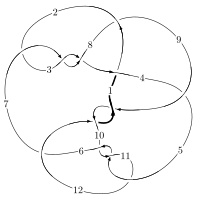
\includegraphics[width=112pt]{../../../GIT/diagram.site/Diagrams/png/1825_12a_1024.png}\\
\ \ \ A knot diagram\footnotemark}&
\allowdisplaybreaks
\textbf{Linearized knot diagam} \\
\cline{2-2}
 &
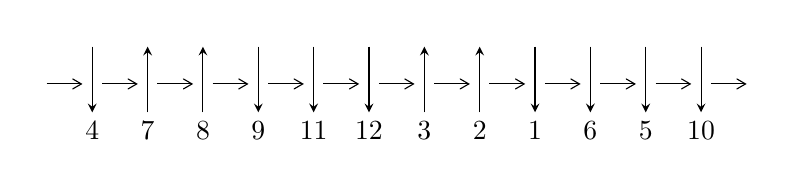
\begin{tikzpicture}[x=20pt, y=17pt]
	% nodes
	\node (C0) at (0, 0) {};
	\node (C1) at (1, 0) {};
	\node (C1U) at (1, +1) {};
	\node (C1D) at (1, -1) {4};

	\node (C2) at (2, 0) {};
	\node (C2U) at (2, +1) {};
	\node (C2D) at (2, -1) {7};

	\node (C3) at (3, 0) {};
	\node (C3U) at (3, +1) {};
	\node (C3D) at (3, -1) {8};

	\node (C4) at (4, 0) {};
	\node (C4U) at (4, +1) {};
	\node (C4D) at (4, -1) {9};

	\node (C5) at (5, 0) {};
	\node (C5U) at (5, +1) {};
	\node (C5D) at (5, -1) {11};

	\node (C6) at (6, 0) {};
	\node (C6U) at (6, +1) {};
	\node (C6D) at (6, -1) {12};

	\node (C7) at (7, 0) {};
	\node (C7U) at (7, +1) {};
	\node (C7D) at (7, -1) {3};

	\node (C8) at (8, 0) {};
	\node (C8U) at (8, +1) {};
	\node (C8D) at (8, -1) {2};

	\node (C9) at (9, 0) {};
	\node (C9U) at (9, +1) {};
	\node (C9D) at (9, -1) {1};

	\node (C10) at (10, 0) {};
	\node (C10U) at (10, +1) {};
	\node (C10D) at (10, -1) {6};

	\node (C11) at (11, 0) {};
	\node (C11U) at (11, +1) {};
	\node (C11D) at (11, -1) {5};

	\node (C12) at (12, 0) {};
	\node (C12U) at (12, +1) {};
	\node (C12D) at (12, -1) {10};
	\node (C13) at (13, 0) {};

	% arrows
	\draw[->,>={angle 60}]
	(C0) edge (C1) (C1) edge (C2) (C2) edge (C3) (C3) edge (C4) (C4) edge (C5) (C5) edge (C6) (C6) edge (C7) (C7) edge (C8) (C8) edge (C9) (C9) edge (C10) (C10) edge (C11) (C11) edge (C12) (C12) edge (C13) ;	\draw[->,>=stealth]
	(C1U) edge (C1D) (C2D) edge (C2U) (C3D) edge (C3U) (C4U) edge (C4D) (C5U) edge (C5D) (C6U) edge (C6D) (C7D) edge (C7U) (C8D) edge (C8U) (C9U) edge (C9D) (C10U) edge (C10D) (C11U) edge (C11D) (C12U) edge (C12D) ;
	\end{tikzpicture} \\
\hhline{~~} \\& 
\textbf{Solving Sequence} \\ \cline{2-2} 
 &
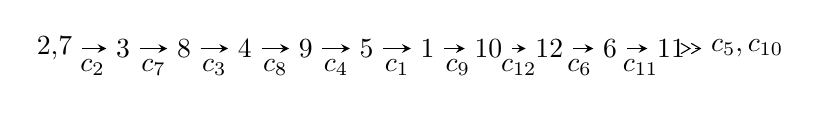
\begin{tikzpicture}[x=22pt, y=7pt]
	% node
	\node (A0) at (-1/8, 0) {2,7};
	\node (A1) at (1, 0) {3};
	\node (A2) at (2, 0) {8};
	\node (A3) at (3, 0) {4};
	\node (A4) at (4, 0) {9};
	\node (A5) at (5, 0) {5};
	\node (A6) at (6, 0) {1};
	\node (A7) at (7, 0) {10};
	\node (A8) at (8, 0) {12};
	\node (A9) at (9, 0) {6};
	\node (A10) at (10, 0) {11};
	\node (C1) at (1/2, -1) {$c_{2}$};
	\node (C2) at (3/2, -1) {$c_{7}$};
	\node (C3) at (5/2, -1) {$c_{3}$};
	\node (C4) at (7/2, -1) {$c_{8}$};
	\node (C5) at (9/2, -1) {$c_{4}$};
	\node (C6) at (11/2, -1) {$c_{1}$};
	\node (C7) at (13/2, -1) {$c_{9}$};
	\node (C8) at (15/2, -1) {$c_{12}$};
	\node (C9) at (17/2, -1) {$c_{6}$};
	\node (C10) at (19/2, -1) {$c_{11}$};
	\node (A11) at (45/4, 0) {$c_{5},c_{10}$};

	% edge
	\draw[->,>=stealth]	
	(A0) edge (A1) (A1) edge (A2) (A2) edge (A3) (A3) edge (A4) (A4) edge (A5) (A5) edge (A6) (A6) edge (A7) (A7) edge (A8) (A8) edge (A9) (A9) edge (A10) ;
	\draw[->>,>={angle 60}]	
	(A10) edge (A11);
\end{tikzpicture} \\ 

\end{tabular} \\

\footnotetext{
The image of knot diagram is generated by the software ``\textbf{Draw programme}" developed by Andrew Bartholomew(\url{http://www.layer8.co.uk/maths/draw/index.htm\#Running-draw}), where we modified some parts for our purpose(\url{https://github.com/CATsTAILs/LinksPainter}).
}\phantom \\ \newline 
\centering \textbf{Ideals for irreducible components\footnotemark of $X_{\text{par}}$} 
 
\begin{align*}
I^u_{1}&=\langle 
u^{74}+u^{73}+\cdots- u+1\rangle \\
\\
\end{align*}
\raggedright * 1 irreducible components of $\dim_{\mathbb{C}}=0$, with total 74 representations.\\
\footnotetext{All coefficients of polynomials are rational numbers. But the coefficients are sometimes approximated in decimal forms when there is not enough margin.}
\newpage
\renewcommand{\arraystretch}{1}
\centering \section*{I. $I^u_{1}= \langle u^{74}+u^{73}+\cdots- u+1 \rangle$}
\flushleft \textbf{(i) Arc colorings}\\
\begin{tabular}{m{7pt} m{180pt} m{7pt} m{180pt} }
\flushright $a_{2}=$&$\begin{pmatrix}1\\0\end{pmatrix}$ \\
\flushright $a_{7}=$&$\begin{pmatrix}0\\u\end{pmatrix}$ \\
\flushright $a_{3}=$&$\begin{pmatrix}1\\- u^2\end{pmatrix}$ \\
\flushright $a_{8}=$&$\begin{pmatrix}u\\- u^3+u\end{pmatrix}$ \\
\flushright $a_{4}=$&$\begin{pmatrix}- u^2+1\\u^4-2 u^2\end{pmatrix}$ \\
\flushright $a_{9}=$&$\begin{pmatrix}- u^3+2 u\\- u^3+u\end{pmatrix}$ \\
\flushright $a_{5}=$&$\begin{pmatrix}- u^{10}+5 u^8-8 u^6+3 u^4+u^2+1\\- u^{10}+4 u^8-5 u^6+2 u^4- u^2\end{pmatrix}$ \\
\flushright $a_{1}=$&$\begin{pmatrix}u^6-3 u^4+2 u^2+1\\- u^8+4 u^6-4 u^4\end{pmatrix}$ \\
\flushright $a_{10}=$&$\begin{pmatrix}u^{17}-8 u^{15}+25 u^{13}-36 u^{11}+19 u^9+4 u^7-2 u^5-4 u^3+u\\- u^{19}+9 u^{17}-32 u^{15}+55 u^{13}-43 u^{11}+9 u^9+4 u^5- u^3+u\end{pmatrix}$ \\
\flushright $a_{12}=$&$\begin{pmatrix}u^{28}-13 u^{26}+\cdots+u^2+1\\- u^{30}+14 u^{28}+\cdots-4 u^4- u^2\end{pmatrix}$ \\
\flushright $a_{6}=$&$\begin{pmatrix}u^{57}-26 u^{55}+\cdots+2 u^3+u\\- u^{59}+27 u^{57}+\cdots- u^3+u\end{pmatrix}$ \\
\flushright $a_{11}=$&$\begin{pmatrix}- u^{50}+23 u^{48}+\cdots+u^2+1\\- u^{50}+22 u^{48}+\cdots-4 u^4- u^2\end{pmatrix}$\\&\end{tabular}
\flushleft \textbf{(ii) Obstruction class $= -1$}\\~\\
\flushleft \textbf{(iii) Cusp Shapes $= -4 u^{72}+132 u^{70}+\cdots-8 u+2$}\\~\\
\newpage\renewcommand{\arraystretch}{1}
\flushleft \textbf{(iv) u-Polynomials at the component}\newline \\
\begin{tabular}{m{50pt}|m{274pt}}
Crossings & \hspace{64pt}u-Polynomials at each crossing \\
\hline $$\begin{aligned}c_{1}\end{aligned}$$&$\begin{aligned}
&u^{74}-15 u^{73}+\cdots-21743 u+1519
\end{aligned}$\\
\hline $$\begin{aligned}c_{2},c_{3},c_{7}\end{aligned}$$&$\begin{aligned}
&u^{74}+u^{73}+\cdots- u+1
\end{aligned}$\\
\hline $$\begin{aligned}c_{4}\end{aligned}$$&$\begin{aligned}
&u^{74}- u^{73}+\cdots-55 u+25
\end{aligned}$\\
\hline $$\begin{aligned}c_{5},c_{10},c_{11}\end{aligned}$$&$\begin{aligned}
&u^{74}- u^{73}+\cdots- u+1
\end{aligned}$\\
\hline $$\begin{aligned}c_{6}\end{aligned}$$&$\begin{aligned}
&u^{74}+u^{73}+\cdots-931 u+457
\end{aligned}$\\
\hline $$\begin{aligned}c_{8}\end{aligned}$$&$\begin{aligned}
&u^{74}-3 u^{73}+\cdots+15 u-1
\end{aligned}$\\
\hline $$\begin{aligned}c_{9},c_{12}\end{aligned}$$&$\begin{aligned}
&u^{74}-11 u^{73}+\cdots-267 u+11
\end{aligned}$\\
\hline
\end{tabular}\\~\\
\newpage\renewcommand{\arraystretch}{1}
\flushleft \textbf{(v) Riley Polynomials at the component}\newline \\
\begin{tabular}{m{50pt}|m{274pt}}
Crossings & \hspace{64pt}Riley Polynomials at each crossing \\
\hline $$\begin{aligned}c_{1}\end{aligned}$$&$\begin{aligned}
&y^{74}+29 y^{73}+\cdots+17219705 y+2307361
\end{aligned}$\\
\hline $$\begin{aligned}c_{2},c_{3},c_{7}\end{aligned}$$&$\begin{aligned}
&y^{74}-67 y^{73}+\cdots+y+1
\end{aligned}$\\
\hline $$\begin{aligned}c_{4}\end{aligned}$$&$\begin{aligned}
&y^{74}+5 y^{73}+\cdots-5975 y+625
\end{aligned}$\\
\hline $$\begin{aligned}c_{5},c_{10},c_{11}\end{aligned}$$&$\begin{aligned}
&y^{74}+69 y^{73}+\cdots+y+1
\end{aligned}$\\
\hline $$\begin{aligned}c_{6}\end{aligned}$$&$\begin{aligned}
&y^{74}+25 y^{73}+\cdots+6053133 y+208849
\end{aligned}$\\
\hline $$\begin{aligned}c_{8}\end{aligned}$$&$\begin{aligned}
&y^{74}-7 y^{73}+\cdots-195 y+1
\end{aligned}$\\
\hline $$\begin{aligned}c_{9},c_{12}\end{aligned}$$&$\begin{aligned}
&y^{74}+61 y^{73}+\cdots+4281 y+121
\end{aligned}$\\
\hline
\end{tabular}\\~\\
\newpage\flushleft \textbf{(vi) Complex Volumes and Cusp Shapes}
$$\begin{array}{c|c|c}  
\text{Solutions to }I^u_{1}& \I (\text{vol} + \sqrt{-1}CS) & \text{Cusp shape}\\
 \hline 
\begin{aligned}
u &= -1.03301\phantom{ +0.000000I}\end{aligned}
 & -1.07564\phantom{ +0.000000I} & \phantom{-0.000000 } 0 \\ \hline\begin{aligned}
u &= \phantom{-}1.044940 + 0.102604 I\end{aligned}
 & \phantom{-}2.61986 + 2.87585 I & \phantom{-0.000000 } 0 \\ \hline\begin{aligned}
u &= \phantom{-}1.044940 - 0.102604 I\end{aligned}
 & \phantom{-}2.61986 - 2.87585 I & \phantom{-0.000000 } 0 \\ \hline\begin{aligned}
u &= -1.156210 + 0.191012 I\end{aligned}
 & \phantom{-}2.43321 - 4.72367 I & \phantom{-0.000000 } 0 \\ \hline\begin{aligned}
u &= -1.156210 - 0.191012 I\end{aligned}
 & \phantom{-}2.43321 + 4.72367 I & \phantom{-0.000000 } 0 \\ \hline\begin{aligned}
u &= \phantom{-}1.158590 + 0.218669 I\end{aligned}
 & \phantom{-}8.21260 + 7.93871 I & \phantom{-0.000000 } 0 \\ \hline\begin{aligned}
u &= \phantom{-}1.158590 - 0.218669 I\end{aligned}
 & \phantom{-}8.21260 - 7.93871 I & \phantom{-0.000000 } 0 \\ \hline\begin{aligned}
u &= \phantom{-}1.196130 + 0.144822 I\end{aligned}
 & \phantom{-}2.98003 + 1.08515 I & \phantom{-0.000000 } 0 \\ \hline\begin{aligned}
u &= \phantom{-}1.196130 - 0.144822 I\end{aligned}
 & \phantom{-}2.98003 - 1.08515 I & \phantom{-0.000000 } 0 \\ \hline\begin{aligned}
u &= \phantom{-}0.320215 + 0.704487 I\end{aligned}
 & \phantom{-}8.01003 + 11.14000 I & \phantom{-}0.39689 - 8.47644 I \\ \hline\begin{aligned}
u &= \phantom{-}0.320215 - 0.704487 I\end{aligned}
 & \phantom{-}8.01003 - 11.14000 I & \phantom{-}0.39689 + 8.47644 I \\ \hline\begin{aligned}
u &= -0.315680 + 0.695529 I\end{aligned}
 & \phantom{-}2.04162 - 7.74964 I & -3.30901 + 8.85384 I \\ \hline\begin{aligned}
u &= -0.315680 - 0.695529 I\end{aligned}
 & \phantom{-}2.04162 + 7.74964 I & -3.30901 - 8.85384 I \\ \hline\begin{aligned}
u &= -0.338213 + 0.679862 I\end{aligned}
 & \phantom{-}8.91437 - 0.94078 I & \phantom{-}1.86731 + 2.75945 I \\ \hline\begin{aligned}
u &= -0.338213 - 0.679862 I\end{aligned}
 & \phantom{-}8.91437 + 0.94078 I & \phantom{-}1.86731 - 2.75945 I \\ \hline\begin{aligned}
u &= \phantom{-}0.320814 + 0.680420 I\end{aligned}
 & \phantom{-}2.53500 + 3.64664 I & -1.83229 - 2.76221 I \\ \hline\begin{aligned}
u &= \phantom{-}0.320814 - 0.680420 I\end{aligned}
 & \phantom{-}2.53500 - 3.64664 I & -1.83229 + 2.76221 I \\ \hline\begin{aligned}
u &= \phantom{-}0.600609 + 0.432783 I\end{aligned}
 & \phantom{-}9.12086 - 7.18945 I & \phantom{-}2.91452 + 2.88104 I \\ \hline\begin{aligned}
u &= \phantom{-}0.600609 - 0.432783 I\end{aligned}
 & \phantom{-}9.12086 + 7.18945 I & \phantom{-}2.91452 - 2.88104 I \\ \hline\begin{aligned}
u &= -1.244690 + 0.203790 I\end{aligned}
 & \phantom{-}8.80185 + 1.44373 I & \phantom{-0.000000 } 0 \\ \hline\begin{aligned}
u &= -1.244690 - 0.203790 I\end{aligned}
 & \phantom{-}8.80185 - 1.44373 I & \phantom{-0.000000 } 0 \\ \hline\begin{aligned}
u &= \phantom{-}0.255238 + 0.678124 I\end{aligned}
 & \phantom{-}1.10543 + 6.03198 I & -4.27580 - 8.07217 I \\ \hline\begin{aligned}
u &= \phantom{-}0.255238 - 0.678124 I\end{aligned}
 & \phantom{-}1.10543 - 6.03198 I & -4.27580 + 8.07217 I \\ \hline\begin{aligned}
u &= -0.545619 + 0.465386 I\end{aligned}
 & \phantom{-}9.78040 - 2.94455 I & \phantom{-}3.94521 + 3.50317 I \\ \hline\begin{aligned}
u &= -0.545619 - 0.465386 I\end{aligned}
 & \phantom{-}9.78040 + 2.94455 I & \phantom{-}3.94521 - 3.50317 I \\ \hline\begin{aligned}
u &= -0.580884 + 0.417872 I\end{aligned}
 & \phantom{-}3.13814 + 3.88721 I & -0.60973 - 3.22333 I \\ \hline\begin{aligned}
u &= -0.580884 - 0.417872 I\end{aligned}
 & \phantom{-}3.13814 - 3.88721 I & -0.60973 + 3.22333 I \\ \hline\begin{aligned}
u &= -0.229715 + 0.657701 I\end{aligned}
 & -3.02571 - 3.01416 I & -10.84049 + 5.92197 I \\ \hline\begin{aligned}
u &= -0.229715 - 0.657701 I\end{aligned}
 & -3.02571 + 3.01416 I & -10.84049 - 5.92197 I \\ \hline\begin{aligned}
u &= \phantom{-}0.544204 + 0.430911 I\end{aligned}
 & \phantom{-}3.50761 + 0.14409 I & \phantom{-}0.63672 - 3.50408 I\\
 \hline 
 \end{array}$$\newpage$$\begin{array}{c|c|c}  
\text{Solutions to }I^u_{1}& \I (\text{vol} + \sqrt{-1}CS) & \text{Cusp shape}\\
 \hline 
\begin{aligned}
u &= \phantom{-}0.544204 - 0.430911 I\end{aligned}
 & \phantom{-}3.50761 - 0.14409 I & \phantom{-}0.63672 + 3.50408 I \\ \hline\begin{aligned}
u &= \phantom{-}0.180185 + 0.648822 I\end{aligned}
 & \phantom{-}0.206108 + 0.208045 I & -6.68575 - 1.16976 I \\ \hline\begin{aligned}
u &= \phantom{-}0.180185 - 0.648822 I\end{aligned}
 & \phantom{-}0.206108 - 0.208045 I & -6.68575 + 1.16976 I \\ \hline\begin{aligned}
u &= \phantom{-}0.043373 + 0.667655 I\end{aligned}
 & \phantom{-}4.86508 - 4.63110 I & -3.42865 + 2.90350 I \\ \hline\begin{aligned}
u &= \phantom{-}0.043373 - 0.667655 I\end{aligned}
 & \phantom{-}4.86508 + 4.63110 I & -3.42865 - 2.90350 I \\ \hline\begin{aligned}
u &= \phantom{-}1.344970 + 0.183030 I\end{aligned}
 & \phantom{-}3.43197 + 1.12512 I & \phantom{-0.000000 } 0 \\ \hline\begin{aligned}
u &= \phantom{-}1.344970 - 0.183030 I\end{aligned}
 & \phantom{-}3.43197 - 1.12512 I & \phantom{-0.000000 } 0 \\ \hline\begin{aligned}
u &= -0.354775 + 0.535609 I\end{aligned}
 & \phantom{-}5.20691 - 1.66335 I & \phantom{-}3.09565 + 4.27561 I \\ \hline\begin{aligned}
u &= -0.354775 - 0.535609 I\end{aligned}
 & \phantom{-}5.20691 + 1.66335 I & \phantom{-}3.09565 - 4.27561 I \\ \hline\begin{aligned}
u &= -0.055516 + 0.627489 I\end{aligned}
 & -0.83877 + 1.62690 I & -7.90840 - 3.45819 I \\ \hline\begin{aligned}
u &= -0.055516 - 0.627489 I\end{aligned}
 & -0.83877 - 1.62690 I & -7.90840 + 3.45819 I \\ \hline\begin{aligned}
u &= \phantom{-}0.592806 + 0.205238 I\end{aligned}
 & \phantom{-}2.64797 - 2.62283 I & -0.82675 + 2.90416 I \\ \hline\begin{aligned}
u &= \phantom{-}0.592806 - 0.205238 I\end{aligned}
 & \phantom{-}2.64797 + 2.62283 I & -0.82675 - 2.90416 I \\ \hline\begin{aligned}
u &= -1.367910 + 0.115025 I\end{aligned}
 & \phantom{-}8.34672 + 1.48194 I & \phantom{-0.000000 } 0 \\ \hline\begin{aligned}
u &= -1.367910 - 0.115025 I\end{aligned}
 & \phantom{-}8.34672 - 1.48194 I & \phantom{-0.000000 } 0 \\ \hline\begin{aligned}
u &= -1.368940 + 0.243993 I\end{aligned}
 & \phantom{-}5.12052 - 3.43600 I & \phantom{-0.000000 } 0 \\ \hline\begin{aligned}
u &= -1.368940 - 0.243993 I\end{aligned}
 & \phantom{-}5.12052 + 3.43600 I & \phantom{-0.000000 } 0 \\ \hline\begin{aligned}
u &= -1.385570 + 0.216376 I\end{aligned}
 & \phantom{-}4.94675 - 3.91535 I & \phantom{-0.000000 } 0 \\ \hline\begin{aligned}
u &= -1.385570 - 0.216376 I\end{aligned}
 & \phantom{-}4.94675 + 3.91535 I & \phantom{-0.000000 } 0 \\ \hline\begin{aligned}
u &= \phantom{-}1.389990 + 0.255951 I\end{aligned}
 & \phantom{-}2.13515 + 6.33953 I & \phantom{-0.000000 } 0 \\ \hline\begin{aligned}
u &= \phantom{-}1.389990 - 0.255951 I\end{aligned}
 & \phantom{-}2.13515 - 6.33953 I & \phantom{-0.000000 } 0 \\ \hline\begin{aligned}
u &= -1.40031 + 0.26526 I\end{aligned}
 & \phantom{-}6.38349 - 9.46596 I & \phantom{-0.000000 } 0 \\ \hline\begin{aligned}
u &= -1.40031 - 0.26526 I\end{aligned}
 & \phantom{-}6.38349 + 9.46596 I & \phantom{-0.000000 } 0 \\ \hline\begin{aligned}
u &= \phantom{-}1.42079 + 0.21110 I\end{aligned}
 & \phantom{-}10.85890 + 4.43876 I & \phantom{-0.000000 } 0 \\ \hline\begin{aligned}
u &= \phantom{-}1.42079 - 0.21110 I\end{aligned}
 & \phantom{-}10.85890 - 4.43876 I & \phantom{-0.000000 } 0 \\ \hline\begin{aligned}
u &= \phantom{-}0.206283 + 0.524313 I\end{aligned}
 & -0.161322 + 1.134130 I & -2.63011 - 5.69236 I \\ \hline\begin{aligned}
u &= \phantom{-}0.206283 - 0.524313 I\end{aligned}
 & -0.161322 - 1.134130 I & -2.63011 + 5.69236 I \\ \hline\begin{aligned}
u &= -1.42841 + 0.26365 I\end{aligned}
 & \phantom{-}8.13467 - 7.09316 I & \phantom{-0.000000 } 0 \\ \hline\begin{aligned}
u &= -1.42841 - 0.26365 I\end{aligned}
 & \phantom{-}8.13467 + 7.09316 I & \phantom{-0.000000 } 0 \\ \hline\begin{aligned}
u &= -1.44510 + 0.14916 I\end{aligned}
 & \phantom{-}9.77486 - 2.20808 I & \phantom{-0.000000 } 0\\
 \hline 
 \end{array}$$\newpage$$\begin{array}{c|c|c}  
\text{Solutions to }I^u_{1}& \I (\text{vol} + \sqrt{-1}CS) & \text{Cusp shape}\\
 \hline 
\begin{aligned}
u &= -1.44510 - 0.14916 I\end{aligned}
 & \phantom{-}9.77486 + 2.20808 I & \phantom{-0.000000 } 0 \\ \hline\begin{aligned}
u &= \phantom{-}1.44646 + 0.13855 I\end{aligned}
 & \phantom{-}9.50233 - 1.95720 I & \phantom{-0.000000 } 0 \\ \hline\begin{aligned}
u &= \phantom{-}1.44646 - 0.13855 I\end{aligned}
 & \phantom{-}9.50233 + 1.95720 I & \phantom{-0.000000 } 0 \\ \hline\begin{aligned}
u &= \phantom{-}1.42809 + 0.27008 I\end{aligned}
 & \phantom{-}7.62286 + 11.27000 I & \phantom{-0.000000 } 0 \\ \hline\begin{aligned}
u &= \phantom{-}1.42809 - 0.27008 I\end{aligned}
 & \phantom{-}7.62286 - 11.27000 I & \phantom{-0.000000 } 0 \\ \hline\begin{aligned}
u &= -1.43094 + 0.27329 I\end{aligned}
 & \phantom{-}13.6165 - 14.7026 I & \phantom{-0.000000 } 0 \\ \hline\begin{aligned}
u &= -1.43094 - 0.27329 I\end{aligned}
 & \phantom{-}13.6165 + 14.7026 I & \phantom{-0.000000 } 0 \\ \hline\begin{aligned}
u &= \phantom{-}1.43495 + 0.26103 I\end{aligned}
 & \phantom{-}14.5965 + 4.3748 I & \phantom{-0.000000 } 0 \\ \hline\begin{aligned}
u &= \phantom{-}1.43495 - 0.26103 I\end{aligned}
 & \phantom{-}14.5965 - 4.3748 I & \phantom{-0.000000 } 0 \\ \hline\begin{aligned}
u &= -1.45330 + 0.13463 I\end{aligned}
 & \phantom{-}15.6001 + 5.2588 I & \phantom{-0.000000 } 0 \\ \hline\begin{aligned}
u &= -1.45330 - 0.13463 I\end{aligned}
 & \phantom{-}15.6001 - 5.2588 I & \phantom{-0.000000 } 0 \\ \hline\begin{aligned}
u &= \phantom{-}1.45302 + 0.15468 I\end{aligned}
 & \phantom{-}16.1228 + 5.1353 I & \phantom{-0.000000 } 0 \\ \hline\begin{aligned}
u &= \phantom{-}1.45302 - 0.15468 I\end{aligned}
 & \phantom{-}16.1228 - 5.1353 I & \phantom{-0.000000 } 0 \\ \hline\begin{aligned}
u &= -0.526726\phantom{ +0.000000I}\end{aligned}
 & -1.25260\phantom{ +0.000000I} & -7.49050\phantom{ +0.000000I}\\
 \hline 
 \end{array}$$\newpage
\newpage\renewcommand{\arraystretch}{1}
\centering \section*{ II. u-Polynomials}
\begin{tabular}{m{50pt}|m{274pt}}
Crossings & \hspace{64pt}u-Polynomials at each crossing \\
\hline $$\begin{aligned}c_{1}\end{aligned}$$&$\begin{aligned}
&u^{74}-15 u^{73}+\cdots-21743 u+1519
\end{aligned}$\\
\hline $$\begin{aligned}c_{2},c_{3},c_{7}\end{aligned}$$&$\begin{aligned}
&u^{74}+u^{73}+\cdots- u+1
\end{aligned}$\\
\hline $$\begin{aligned}c_{4}\end{aligned}$$&$\begin{aligned}
&u^{74}- u^{73}+\cdots-55 u+25
\end{aligned}$\\
\hline $$\begin{aligned}c_{5},c_{10},c_{11}\end{aligned}$$&$\begin{aligned}
&u^{74}- u^{73}+\cdots- u+1
\end{aligned}$\\
\hline $$\begin{aligned}c_{6}\end{aligned}$$&$\begin{aligned}
&u^{74}+u^{73}+\cdots-931 u+457
\end{aligned}$\\
\hline $$\begin{aligned}c_{8}\end{aligned}$$&$\begin{aligned}
&u^{74}-3 u^{73}+\cdots+15 u-1
\end{aligned}$\\
\hline $$\begin{aligned}c_{9},c_{12}\end{aligned}$$&$\begin{aligned}
&u^{74}-11 u^{73}+\cdots-267 u+11
\end{aligned}$\\
\hline
\end{tabular}\newpage\renewcommand{\arraystretch}{1}
\centering \section*{ III. Riley Polynomials}
\begin{tabular}{m{50pt}|m{274pt}}
Crossings & \hspace{64pt}Riley Polynomials at each crossing \\
\hline $$\begin{aligned}c_{1}\end{aligned}$$&$\begin{aligned}
&y^{74}+29 y^{73}+\cdots+17219705 y+2307361
\end{aligned}$\\
\hline $$\begin{aligned}c_{2},c_{3},c_{7}\end{aligned}$$&$\begin{aligned}
&y^{74}-67 y^{73}+\cdots+y+1
\end{aligned}$\\
\hline $$\begin{aligned}c_{4}\end{aligned}$$&$\begin{aligned}
&y^{74}+5 y^{73}+\cdots-5975 y+625
\end{aligned}$\\
\hline $$\begin{aligned}c_{5},c_{10},c_{11}\end{aligned}$$&$\begin{aligned}
&y^{74}+69 y^{73}+\cdots+y+1
\end{aligned}$\\
\hline $$\begin{aligned}c_{6}\end{aligned}$$&$\begin{aligned}
&y^{74}+25 y^{73}+\cdots+6053133 y+208849
\end{aligned}$\\
\hline $$\begin{aligned}c_{8}\end{aligned}$$&$\begin{aligned}
&y^{74}-7 y^{73}+\cdots-195 y+1
\end{aligned}$\\
\hline $$\begin{aligned}c_{9},c_{12}\end{aligned}$$&$\begin{aligned}
&y^{74}+61 y^{73}+\cdots+4281 y+121
\end{aligned}$\\
\hline
\end{tabular}
\vskip 2pc
\end{document}